\documentclass[fr]{../../../../../../eplexam}
\usepackage{float}
\usepackage{mathtools}
\usepackage{tikz}
\usepackage{enumitem}
\usepackage{graphicx}
\usepackage{caption}
\usepackage{multicol}

\usepackage{../../../../../../eplcode}
\lstset{language={C}}

\hypertitle{Systèmes informatiques}{4}{SINF}{1252}{2017}{Juin}{Majeure}
{Quentin Dessain \and Gilles Peiffer \and Thomas Reniers}
{Olivier Bonaventure}


\section{Exécution conditionnelle [4 points]}
Le shell \texttt{bash} permet l'exécution conditionnelle de commandes. Celle-ci est décrite comme suit dans la page de manuel de \texttt{bash}:

\vspace{0.2cm}
\texttt{An OR list has the form}

\vspace{0.05cm}
\texttt{command1} $\vert\vert$ \texttt{command2}

\vspace{0.05cm}
\texttt{command2 is executed if and only if command1 returns a non-zero exit status.The return status of AND and OR lists is the exit status of the last command executed in the list.}
\vspace{0.01cm}

Expliquez en détail \textbf{tous} les appels système utilisés \textbf{par le shell} lors de l'éxecution de la ligne de commande \texttt{bash} suivante:
\vspace{0.01cm}

\texttt{/bin/prog \textgreater/tmp/t  $\vert\vert$ /bin/prog2}

\begin{solution}

\begin{center}
  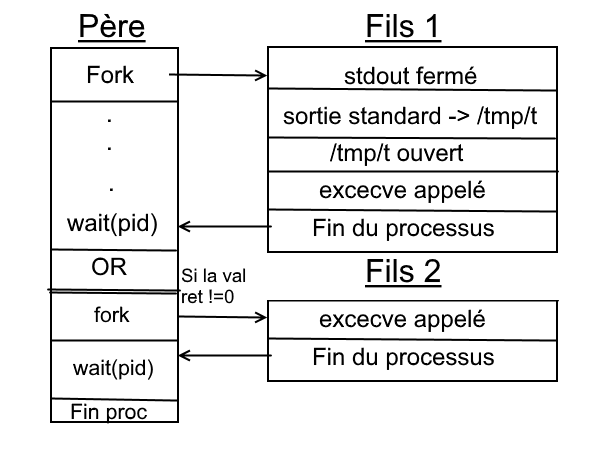
\includegraphics[width=0.6 \textwidth]{latex.png}
\end{center}

Pour le processus père:
\begin{itemize}
\item Un appel système vers \texttt{fork} est effectué, ce qui a pour effet de créer un processus fils (processus fils 1).
    \item Un appel vers \texttt{wait(pid)} ``bloque'' le processus père tant que le fils n'a pas terminé.
    \item La valeur de retour du fils est testée. Si la valeur retournée est différente de zéro, un nouveau processus fils (processus fils 2) est créé.
    \item Si un nouveau processus fils est créé, un appel vers \texttt{wait(pid)} ``bloque'' le processus père tant que le fils n'est pas terminé.
\end{itemize}

Pour le processus fils 1:
\begin{itemize}

\item Une fois le processus fils créé, la sortie standard \texttt{stdout} est fermée.

\item Ensuite, la sortie standard du processus fils est redirigée vers le fichier \texttt{/tmp/t}. Si ce dernier n'existait pas, il est créé. Si il existait déjà, il est remis à zéro.

\item Le fichier \texttt{/tmp/t} est ouvert afin de pouvoir écrire dedans.

\item \texttt{execve} est appélé et le processus situé dans \texttt{/bin/prog} est lancé.

\item Le processus se termine. (Pas d'appel système ? Quid de la nouvelle sortie standard ? Est-elle fermée ?)

\end{itemize}



Pour le processus fils 2:
\begin{itemize}
    \item \texttt{execve} est appélé et le processus situé dans \texttt{/bin/prog2} est lancé.
\end{itemize}



\end{solution}
\section{Mémoire virtuelle [3 points]}


Considérons un processus qui s'exécute sur un ordinateur utilisant la mémoire virtuelle. Pour simplifier, supposons que ce processus utilise une page pour son segment de code, une page pour ses variables globales, une page pour son \textit{heap} et une page pour son \textit{stack}. Ce processus, dans sa fonction \texttt{main}, exécute les lignes suivantes:

\begin{lstlisting}
int main(int argc, char** argv){
int *ptr =(int *) malloc(sizeof(int));
*ptr = 1252;
}
\end{lstlisting}


\begin{itemize}


\item[$\bullet$] Expliquez l'organisation du processus en mémoire et indiquez dans quelles zones se trouvent le code des fonctions \texttt{main} et \texttt{malloc}, la variable \texttt{*ptr} et la zone mémoire retournée par \texttt{malloc}.

\begin{solution}

\begin{multicols}{2}
    \begin{center}
         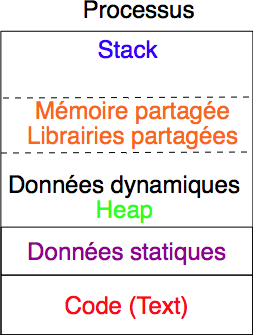
\includegraphics[width=0.4 \textwidth]{orgMemoire.png}
          \captionof{figure}{Organisation en mémoire d’un processus.}
     \end{center}
    \begin{center}
         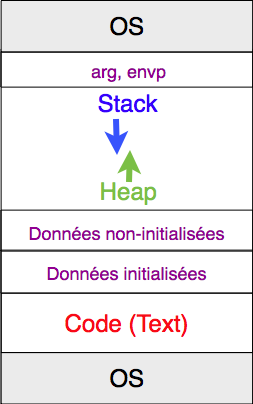
\includegraphics[width=0.3 \textwidth]{figures-001-c.png}
          \captionof{figure}{Organisation d’un programme Linux en mémoire.}
     \end{center}
\end{multicols}


C’est dans le \textbf{segment text} que sont stockées toutes les instructions qui sont exécutées par le microprocesseur.
Il est généralement considéré par l’OS comme étant uniquement
accessible en lecture. C’est dans le \textit{segment text} qu’on retrouvera les instructions de langage machine correspondant aux fonctions de calcul et d’affichage du programme.\par
Le code de la fonction \texttt{main} se trouve donc ici.
La fonction \texttt{malloc} se trouve dans la mémoire des librairies partagées, soit dans le \textit{segment text} avec les autres fonctions si la compilation est statique (paramètre \texttt{-static} lors de l'appel à \texttt{gcc}).
\newline

C’est dans la \textbf{pile} (\textbf{stack)} que le processus va stocker l’ensemble des variables locales mais
également les valeurs de retour de toutes les fonctions qui sont appelées. Cette zone est gérée comme
une pile (d’où son nom) avec un fonctionnement de type LIFO (\textit{Last In, First Out}). À chaque
fois qu’une fonction est appelée elle est placée sur la pile ainsi que ses arguments. Les variables locales
le sont également. Durant son exécution, une fonction accède donc à ses variables locales sur la pile sans
interférer avec les variables locales de l’exécution des autres fonctions. \par
La variable \texttt{*ptr} est placée sur la pile.
\newline

Le \textbf{tas} (ou \textbf{heap}) est une des deux zones dans laquelle un
programme peut obtenir de la mémoire supplémentaire pour stocker de l’information. L’OS mémorise
pour chaque processus en cours d’exécution la limite supérieure de son heap et permet à un processus
de modifier la taille de son heap. En \clang{}, la plupart des processus allouent et libèrent de la mémoire en utilisant les
fonctions \texttt{malloc} et \texttt{free} qui font partie de la librairie standard.\par
La zone de mémoire retournée par \texttt{malloc} est donc située sur le \textit{heap}.
\newline

Le segment des données initialisées contient l’ensemble des données et chaînes de caractères qui sont utilisées
dans le programme. Ce segment contient 2 types de données :
\begin{itemize}
     \item l’ensemble des variables globales qui sont explicitement initialisées
     par le programme ou initialisées à 0 par le compilateur;
     \item les constantes et chaînes de caractères utilisées par le programme.
\end{itemize}

Le segment des données non initialisées est réservé aux variables non initialisées. Cette zone en mémoire est initialisée à zéro par l’OS au démarrage du programme.

\end{solution}

\item[$\bullet$] Dessinez la table des pages de ce processus avec les valeurs des différents drapeaux au démarrage du processus. Expliquez le rôle de ces drapeaux.

\begin{solution}
\begin{table}[H]
\centering
\label{my-label}
\begin{tabular}{|c|l|l|l|l|l|}
\hline
Page & \multicolumn{1}{c|}{\begin{tabular}[c]{@{}c@{}}Bit de \\ référence\end{tabular}} & \multicolumn{1}{c|}{\begin{tabular}[c]{@{}c@{}}Bit de \\ modification\\ (\textit{dirty bit})\end{tabular}} & \multicolumn{1}{c|}{\begin{tabular}[c]{@{}c@{}}Bit de \\ permission \\ (R-W-X)\end{tabular}} & \multicolumn{1}{c|}{\begin{tabular}[c]{@{}c@{}}Bit de \\ validité\end{tabular}} & \multicolumn{1}{c|}{\begin{tabular}[c]{@{}c@{}}Localisation \\ de la page\end{tabular}} \\ \hline
\multicolumn{6}{|c|}{État à la ligne 1 du code} \\ \hline
Segment Text & \texttt{TRUE} & \texttt{FALSE} & R - X & Inchangé &  \\ \hline
Variables Globales & \texttt{FALSE} & \texttt{FALSE} & R - W & Inchangé &  \\ \hline
Heap & \texttt{TRUE} & \texttt{FALSE} & R - W & Inchangé &  \\ \hline
Stack & \texttt{TRUE} & \texttt{FALSE} & R - W & Inchangé &  \\ \hline
\multicolumn{6}{|c|}{État à la ligne 2 du code} \\ \hline
Segment Text & \texttt{TRUE} & \texttt{FALSE} & R - X & Inchangé &  \\ \hline
Variables Globales & \texttt{FALSE} & \texttt{FALSE} & R - W & Inchangé &  \\ \hline
Heap & \texttt{TRUE} & \texttt{TRUE} & R - W & Inchangé &  \\ \hline
Stack & \texttt{TRUE} & \texttt{TRUE} & R - W & Inchangé &  \\ \hline
\multicolumn{6}{|c|}{État à la ligne 3 du code} \\ \hline
Segment Text & \texttt{TRUE} & \texttt{FALSE} & R - X & Inchangé &  \\ \hline
Variables Globales & \texttt{FALSE} & \texttt{FALSE} & R - W & Inchangé &  \\ \hline
Heap & \texttt{TRUE} & \texttt{TRUE} & R - W & Inchangé &  \\ \hline
Stack & \texttt{TRUE} & \texttt{TRUE} & R - W & Inchangé &  \\ \hline
\end{tabular}
\end{table}

\begin{itemize}
    \item Bit de référence: indique si la page a été lue.
    \item Bit de modification (\textit{dirty bit}): indique si la page a été lue.
    \item Bit de permission (R, W, X): indique si la page est accessible en lecture/écriture/exécution.
    \item Bit de validité: indique si la page est présente en RAM ou sur l’espace d’échange (\textit{swap}).
\end{itemize}

\end{solution}

\end{itemize}

\section{Algorithme de Peterson [3 points]}

Un site Internet propose l'implémentation suivante pour résoudre le problème de l'exclusion mutuelle en \clang{}. Cette implémentation est-elle correcte? Si oui, justifiez en détail l'absence de \textit{deadlock} et de violation de section critique. Si non, expliquez via un exemple pourquoi elle ne fonctionne pas et proposez une correction en utilisant les mêmes variables.

\begin{lstlisting}

// Initialisation
int a = false;
int b = false;
int c = 0;

// Thread 0
a = true;
c = 0;

while (b || (c == 1)) {}
section_critique();
a = false;

// Thread 1
b = true;
c = 1;
while (a || (c == 0)) {}
section_critique();
b = false;

\end{lstlisting}

\begin{solution}
Cette implémentation est incorrecte et conduit à un \textit{deadlock}.
\newline

\paragraph{Exemple}
Les 2 premières lignes du premier thread sont executées suivi des 3 premières lignes du deuxième thread. Ensuite, la troisième ligne du premier thread est éxecutée.
\par
Les threads 1 et 2 sont alors tous les deux bloqués dans une boucle infinie sans qu'un thread ne puisse libérer l'autre. On est donc bien face à un \textit{deadlock}.

Voici une implémentation correcte de l'algorithme de Peterson.

\begin{lstlisting}

// Initialisation
int a = false;
int b = false;
int c;

// Thread 0
a = true;
c = 1;

while (b || (c == 1)) {}

section_critique();

a = false;

// Thread 1
b = true;
c = 0;
while (a || (c == 0)) {}

section_critique();

b = false;

\end{lstlisting}

Cette solution ne provoque pas de \textit{deadlock}, de \textit{livelock} ni de violation de section critique et satisfait aux 3 critères de solution du problème de violation de section critique.

\end{solution}

Le syllabus est accessible depuis l'URL \url{http://sites.uclouvain.be/SystInfo}.

\textbf{Les pages de manuel sont accessibles depuis les URLs suivants :}
\begin{itemize}
     \item \url{http://sites.uclouvain.be/SystInfo/manpages/man1} (commandes);
     \item \url{http://sites.uclouvain.be/SystInfo/manpages/man2} (appels systèmes);
     \item \url{http://sites.uclouvain.be/SystInfo/manpages/man3} (fonctions librairies).
\end{itemize}

\textbf{Attention:} veuillez utiliser la version \textbf{\html{}} du syllabus.

\section{Insertion de données dans un fichier}

Les fonctions \texttt{read} et \texttt{write} de lire et d'écrire
des données dans un fichier. Certaines applications doivent parfois insérer
des données dans un fichier à une position précise du fichier en décalant les données
déjà présentes vers la fin du fichier.
Vous devez écrire la fonction \texttt{insert}, dont les spécifications sont reprises
ci-dessous en utilisant les appels système \texttt{read}, \texttt{write}, \texttt{open}, \texttt{close} et \texttt{lseek}.

\begin{lstlisting}
/*
 * @pre fileName!=NULL, buf!=NULL, nbyte >0
 * @post a inséreé dans le fichier filename les nbytes du buffers buf
 *       à la position pos. Les bytes suivants dans le fichiers ont
 *       étés décalées vers la fin du fichier
 *       retourne le nombre de bytes écrites, -1 en cas d'erreur
 */
int insert(char *fileName, off_t pos, const void *buf, size_t nbyte) {
\end{lstlisting}

\begin{solution}

\begin{lstlisting}
int fd = open(fileName,O_RDWR);
if(fd==-1)
{
    return -1;
}
off_t end = lseek(fd,0,SEEK_END);
off_t offset = lseek(fd,pos,SEEK_SET);
off_t toRead = end - offset;
void* toWrite = malloc(toRead); if(toWrite==NULL){return -1;}
if(offset==-1||end==-1)
{
    free(toWrite);
    close(fd);
    return -1;
}
ssize_t red = read(fd,toWrite,(size_t)toRead);
if(red==-1)
{
    free(toWrite);
    close(fd);
    return -1;
}
offset = lseek(fd,pos,SEEK_SET);
if(offset==-1)
{
    free(toWrite);
    close(fd);
    return -1;
}
ssize_t written = write(fd,buf,nbyte);
if(written==-1)
{
    free(toWrite);
    close(fd);
    return -1;
}
ssize_t shift = write(fd,toWrite,(size_t)toRead);
if(shift==-1)
{
    free(toWrite);
    close(fd);
    return -1;
}
free(toWrite);
close(fd);
return written;

\end{lstlisting}

\end{solution}

% TODO Missing exercises.

\end{document}
